\newpage
\chapter{Cell-by-cell reweighting}
In liaison with Section \ref{gamma:ss:reweighting:photon}, additional control plots are shown here.
\section{Electron reweighting applied to photons}
\label{Adx1:Electron}
Figures \ref{Electron:1}, \ref{Electron:2}, \ref{Electron:3} and \ref{Electron:4} show the energy profiles and shower shape variables for 4 $|\eta|$ bins after applying the derived reweighting for electrons on photons. Similar behaviour is observed for the rest of $|\eta|$ bins.  
\begin{figure}[ht]
    \centering
	\subfloat[][]{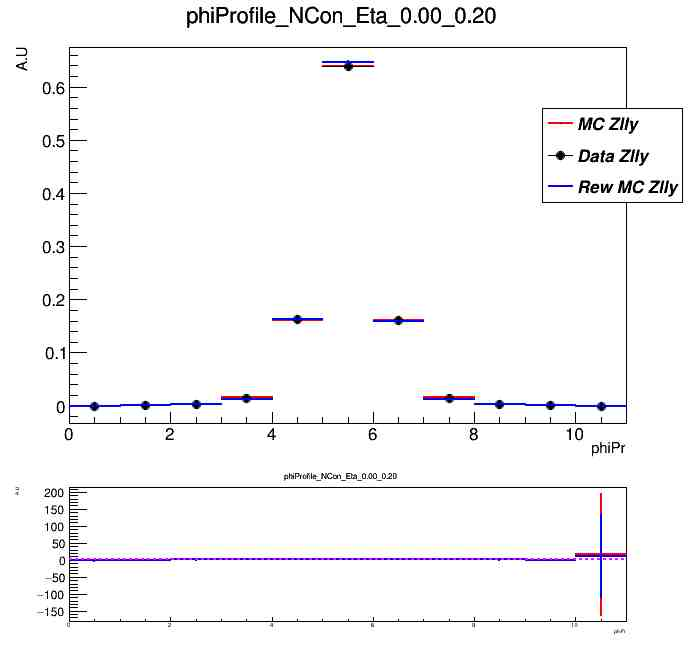
\includegraphics[width=.35\textwidth]{Adx/Adx1/Img/Electron/phiProfileRew_NCon_Eta_0.00_0.20Zlly.jpg}}
	\subfloat[][]{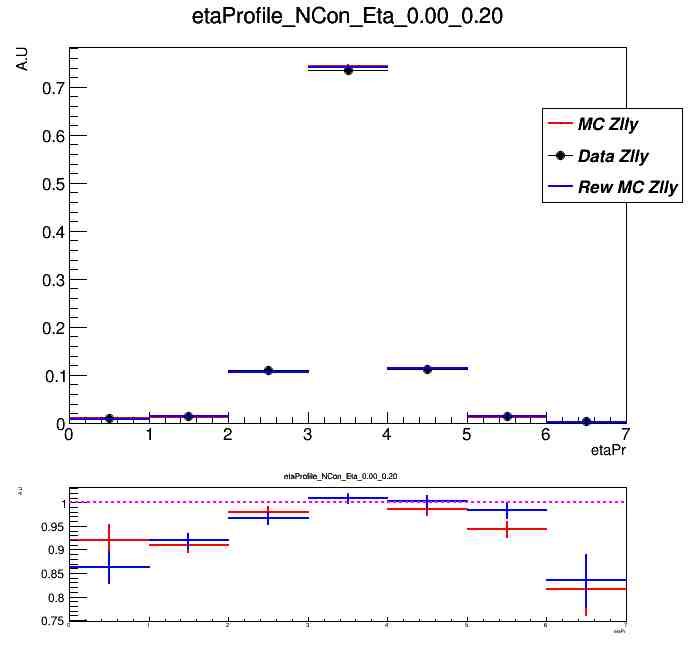
\includegraphics[width=.35\textwidth]{Adx/Adx1/Img/Electron/etaProfileRew_NCon_Eta_0.00_0.20Zlly.jpg}} \\
	\subfloat[][]{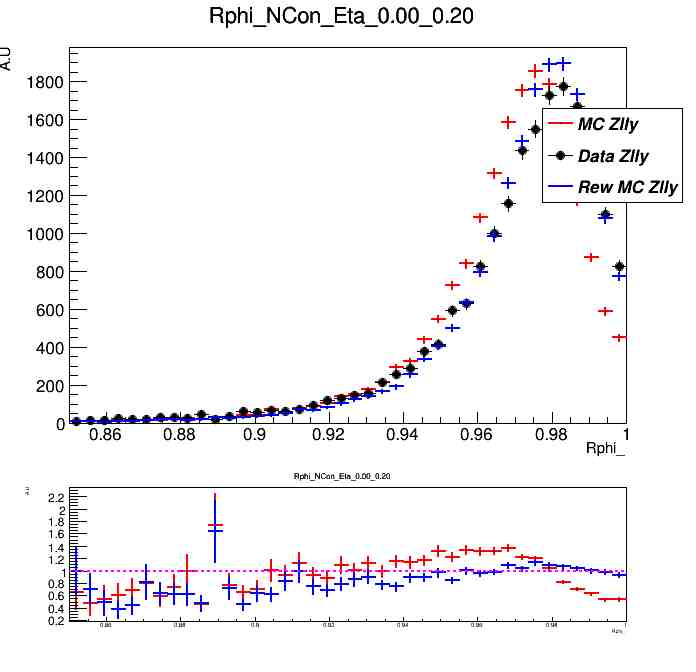
\includegraphics[width=.35\textwidth]{Adx/Adx1/Img/Electron/RphiRew_NCon_Eta_0.00_0.20Zlly.jpg}}
	\subfloat[][]{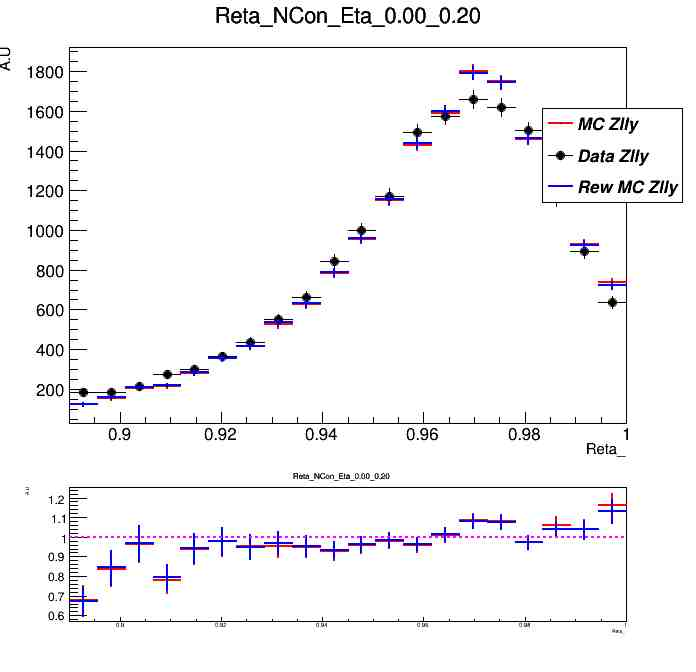
\includegraphics[width=.35\textwidth]{Adx/Adx1/Img/Electron/RetaRew_NCon_Eta_0.00_0.20Zlly.jpg}}
    \caption{The energy profile in $\phi$ and $\eta$ directions (a,b) and the corresponding \Rphi \ and \Reta \ variables, for unconverted photons with 0.00$<|\eta|<$0.20. The black points correspond to the pseudo data, red points to non-reweighted simulation and blue points to the reweighted simulation from $Z\rightarrow ll\gamma$ with derived electron reweighting.}
    \label{Electron:1}
\end{figure}
\begin{figure}[ht]
    \centering
	\subfloat[][]{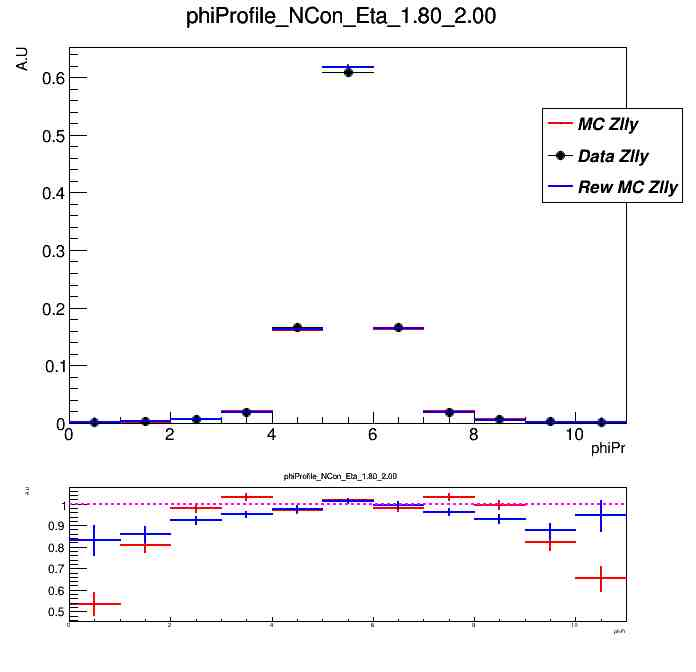
\includegraphics[width=.35\textwidth]{Adx/Adx1/Img/Electron/phiProfileRew_NCon_Eta_1.80_2.00Zlly.jpg}}
	\subfloat[][]{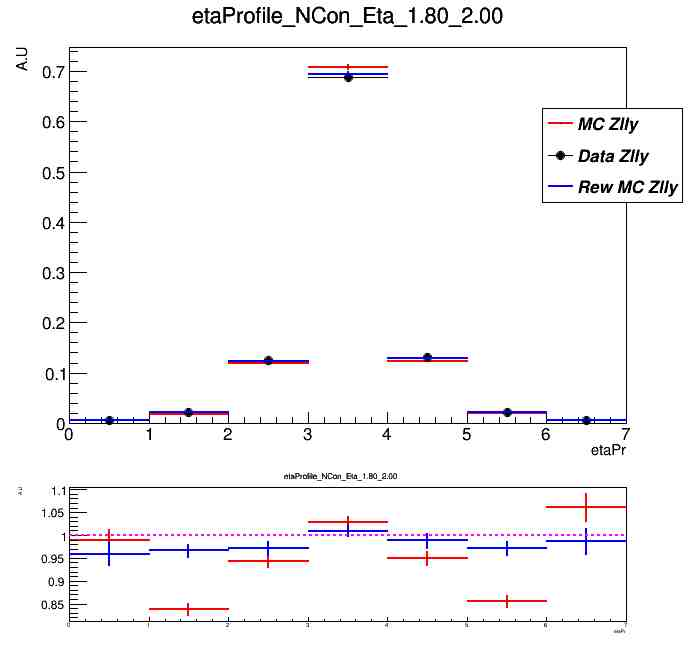
\includegraphics[width=.35\textwidth]{Adx/Adx1/Img/Electron/etaProfileRew_NCon_Eta_1.80_2.00Zlly.jpg}} \\
	\subfloat[][]{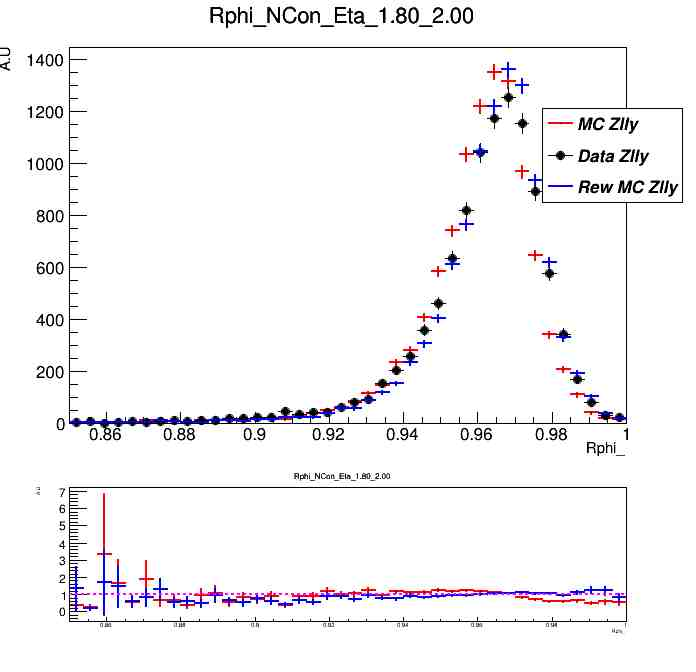
\includegraphics[width=.35\textwidth]{Adx/Adx1/Img/Electron/RphiRew_NCon_Eta_1.80_2.00Zlly.jpg}}
	\subfloat[][]{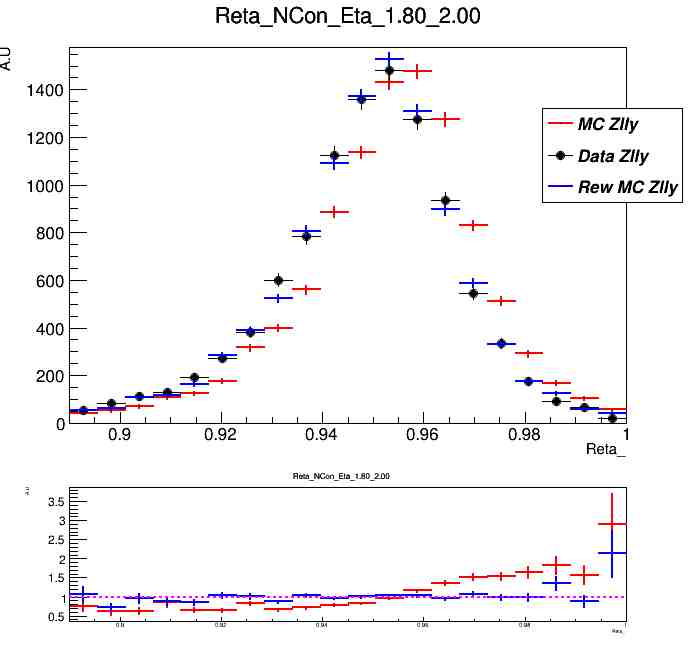
\includegraphics[width=.35\textwidth]{Adx/Adx1/Img/Electron/RetaRew_NCon_Eta_1.80_2.00Zlly.jpg}}
    \caption{The energy profile in $\phi$ and $\eta$ directions (a,b) and the corresponding \Rphi \ and \Reta \ variables, for unconverted photons with 1.80$<|\eta|<$2.00. The black points correspond to the pseudo data, red points to non-reweighted simulation and blue points to the reweighted simulation from $Z\rightarrow ll\gamma$ with derived electron reweighting.}
    \label{Electron:2}
\end{figure}

\begin{figure}[ht]
    \centering
	\subfloat[][]{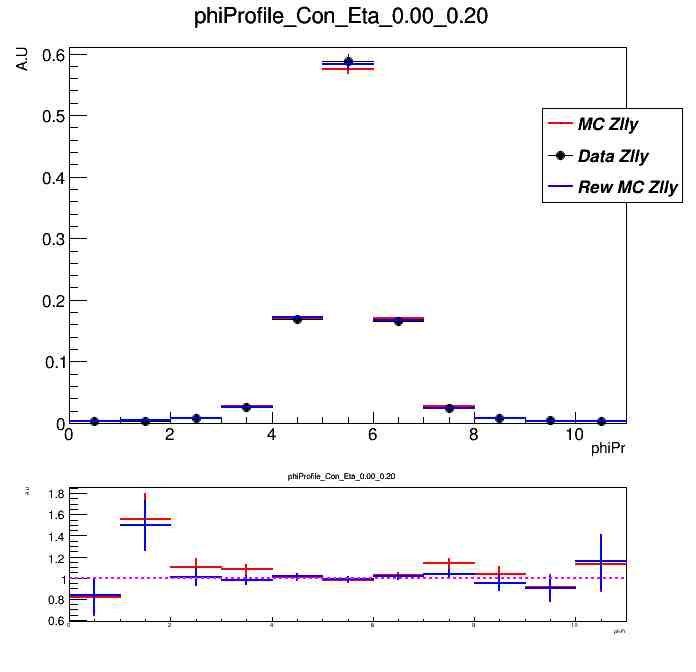
\includegraphics[width=.35\textwidth]{Adx/Adx1/Img/Electron/phiProfileRew_Con_Eta_0.00_0.20Zlly.jpg}}
	\subfloat[][]{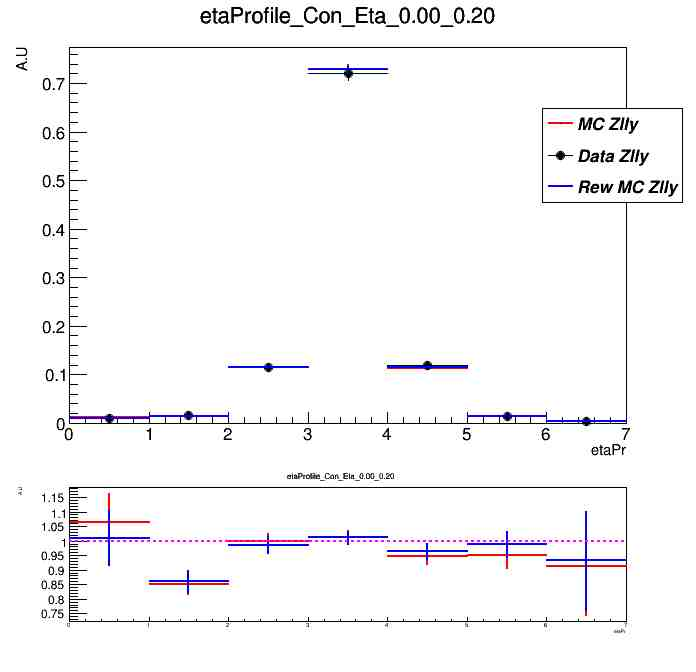
\includegraphics[width=.35\textwidth]{Adx/Adx1/Img/Electron/etaProfileRew_Con_Eta_0.00_0.20Zlly.jpg}} \\
	\subfloat[][]{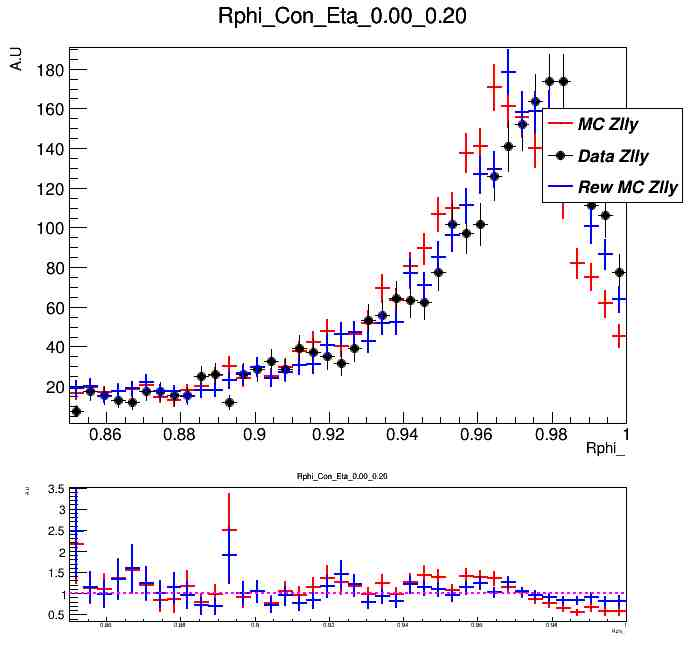
\includegraphics[width=.35\textwidth]{Adx/Adx1/Img/Electron/RphiRew_Con_Eta_0.00_0.20Zlly.jpg}}
	\subfloat[][]{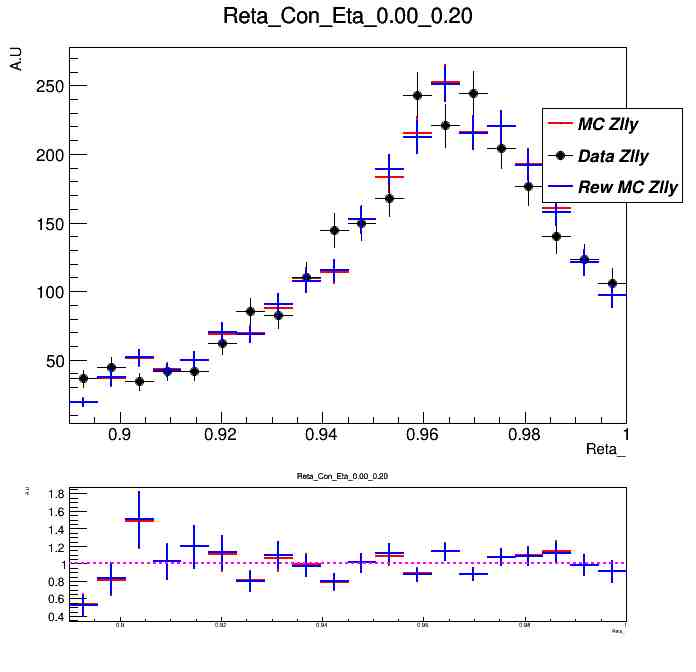
\includegraphics[width=.35\textwidth]{Adx/Adx1/Img/Electron/RetaRew_Con_Eta_0.00_0.20Zlly.jpg}}
    \caption{The energy profile in $\phi$ and $\eta$ directions (a,b) and the corresponding \Rphi \ and \Reta \ variables, for converted photons with 0.00$<|\eta|<$0.20. The black points correspond to the pseudo data, red points to non-reweighted simulation and blue points to the reweighted simulation from $Z\rightarrow ll\gamma$ with derived electron reweighting.}
    \label{Electron:3}
\end{figure}

\begin{figure}[ht]
    \centering
	\subfloat[][]{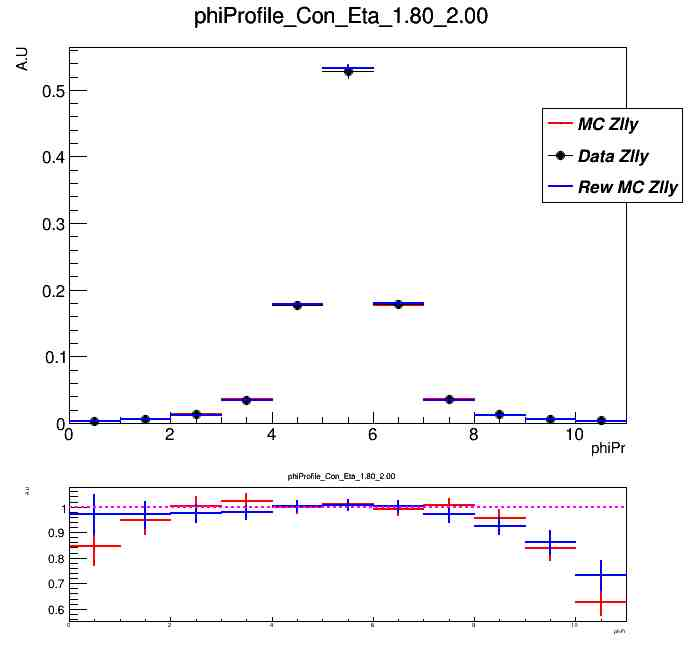
\includegraphics[width=.35\textwidth]{Adx/Adx1/Img/Electron/phiProfileRew_Con_Eta_1.80_2.00Zlly.jpg}}
	\subfloat[][]{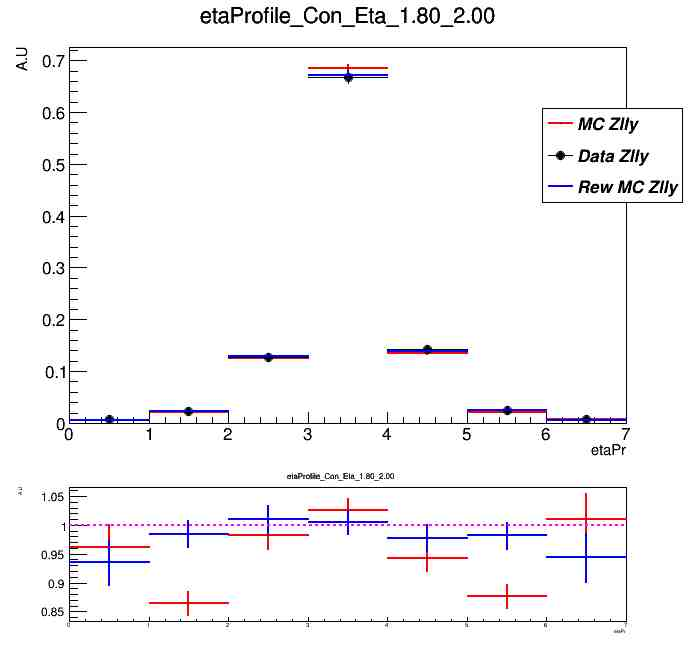
\includegraphics[width=.35\textwidth]{Adx/Adx1/Img/Electron/etaProfileRew_Con_Eta_1.80_2.00Zlly.jpg}} \\
	\subfloat[][]{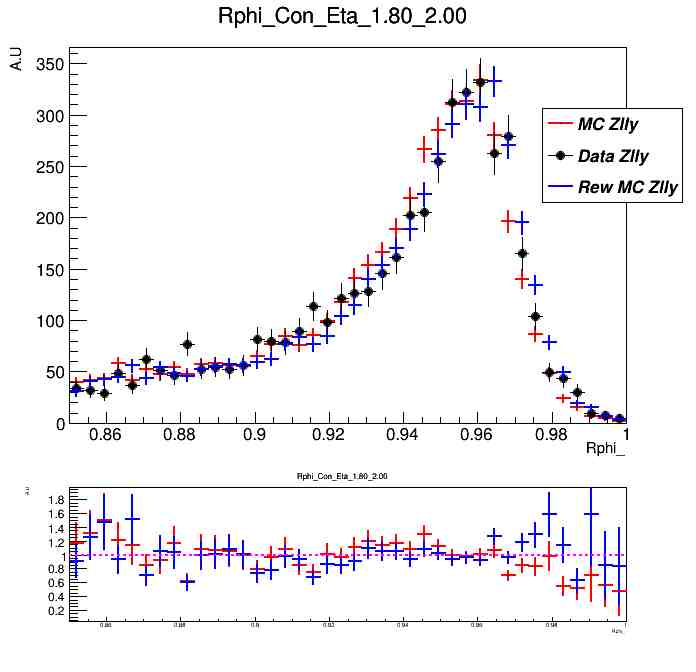
\includegraphics[width=.35\textwidth]{Adx/Adx1/Img/Electron/RphiRew_Con_Eta_1.80_2.00Zlly.jpg}}
	\subfloat[][]{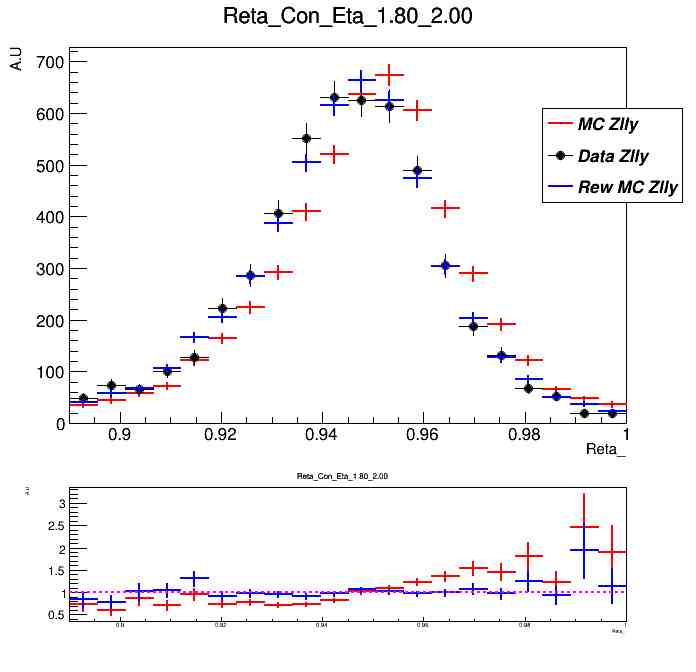
\includegraphics[width=.35\textwidth]{Adx/Adx1/Img/Electron/RetaRew_Con_Eta_1.80_2.00Zlly.jpg}}
    \caption{The energy profile in $\phi$ and $\eta$ directions (a,b) and the corresponding \Rphi \ and \Reta \ variables, for converted photons with 1.80$<|\eta|<$2.00. The black points correspond to the pseudo data, red points to non-reweighted simulation and blue points to the reweighted simulation from $Z\rightarrow ll\gamma$ with derived electron reweighting.}
    \label{Electron:4}
\end{figure}

\section{Specific photon reweighting}
\label{Adx1:Photon}

Figures \ref{Photon:1}, \ref{Photon:2}, \ref{Photon:3} and \ref{Photon:4} show the energy profiles and shower shape variables for 4 $|\eta|$ bins after applying the photon reweighting. Similar behaviour is observed for the rest of $|\eta|$ bins.  
\begin{figure}[ht]
    \centering
	\subfloat[][]{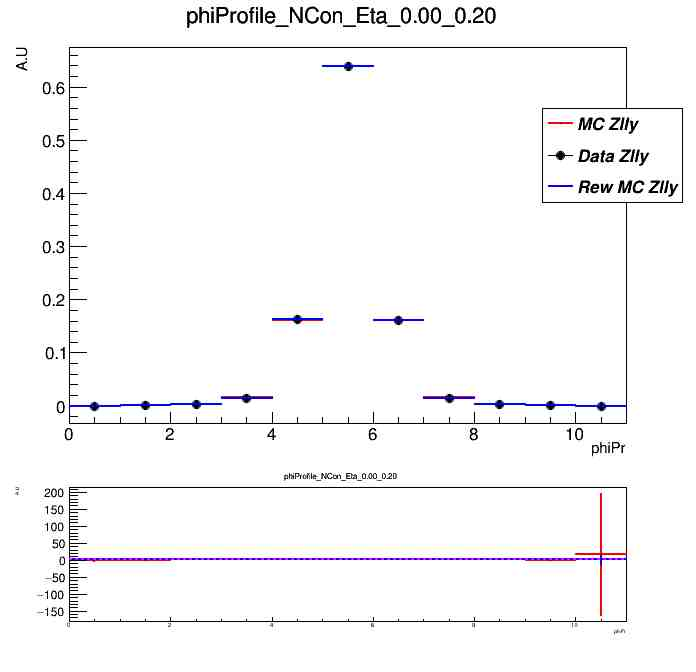
\includegraphics[width=.35\textwidth]{Adx/Adx1/Img/Photon/phiProfileRew_NCon_Eta_0.00_0.20Zlly.jpg}}
	\subfloat[][]{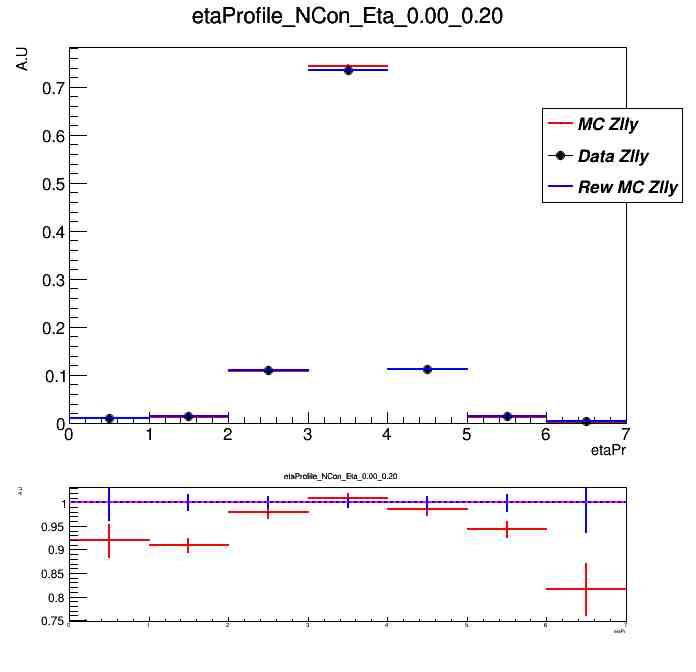
\includegraphics[width=.35\textwidth]{Adx/Adx1/Img/Photon/etaProfileRew_NCon_Eta_0.00_0.20Zlly.jpg}} \\
	\subfloat[][]{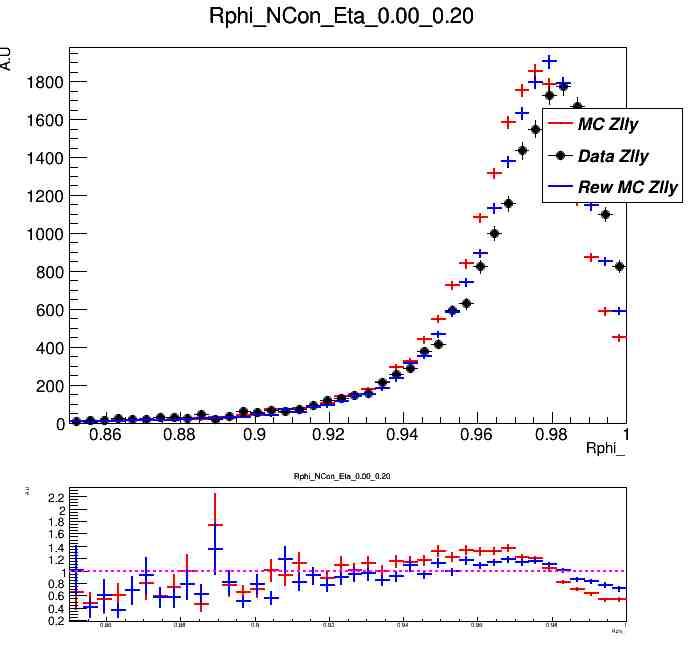
\includegraphics[width=.35\textwidth]{Adx/Adx1/Img/Photon/RphiRew_NCon_Eta_0.00_0.20Zlly.jpg}}
	\subfloat[][]{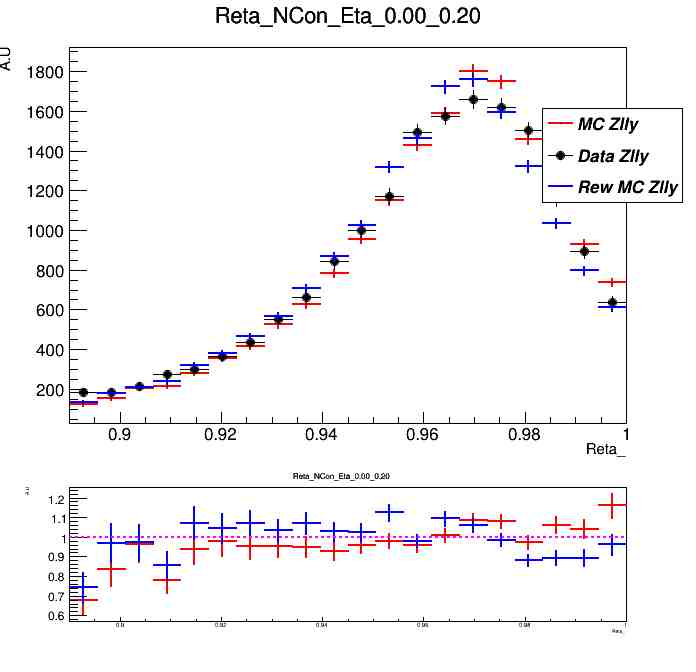
\includegraphics[width=.35\textwidth]{Adx/Adx1/Img/Photon/RetaRew_NCon_Eta_0.00_0.20Zlly.jpg}}
    \caption{The energy profile in $\phi$ and $\eta$ directions (a,b) and the corresponding \Rphi \ and \Reta \ variables, for unconverted photons with 0.00$<|\eta|<$0.20. The black points correspond to the pseudo data, red points to non-reweighted simulation and blue points to the reweighted simulation from $Z\rightarrow ll\gamma$ with derived photon reweighting.}
    \label{Photon:1}
\end{figure}
\begin{figure}[ht]
    \centering
	\subfloat[][]{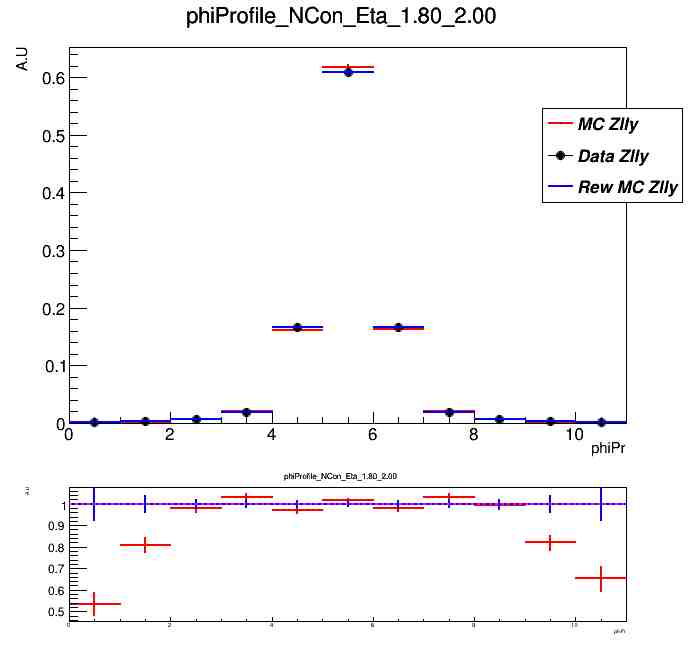
\includegraphics[width=.35\textwidth]{Adx/Adx1/Img/Photon/phiProfileRew_NCon_Eta_1.80_2.00Zlly.jpg}}
	\subfloat[][]{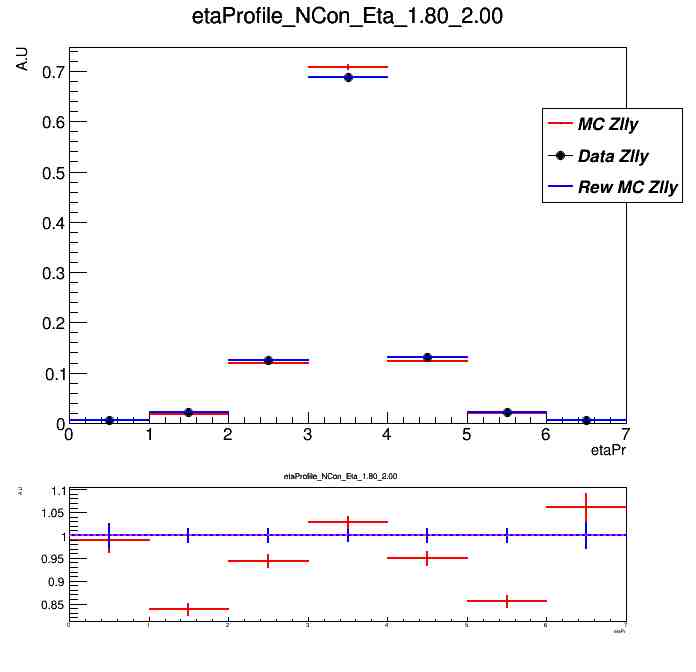
\includegraphics[width=.35\textwidth]{Adx/Adx1/Img/Photon/etaProfileRew_NCon_Eta_1.80_2.00Zlly.jpg}} \\
	\subfloat[][]{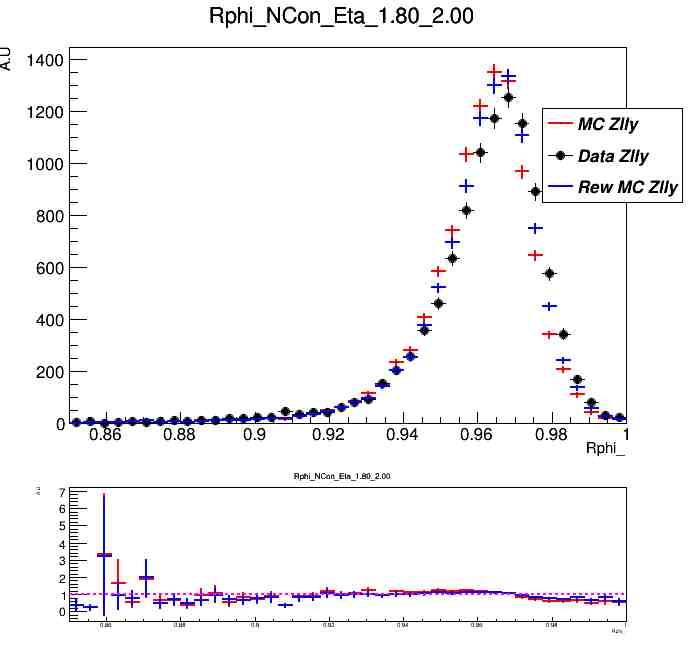
\includegraphics[width=.35\textwidth]{Adx/Adx1/Img/Photon/RphiRew_NCon_Eta_1.80_2.00Zlly.jpg}}
	\subfloat[][]{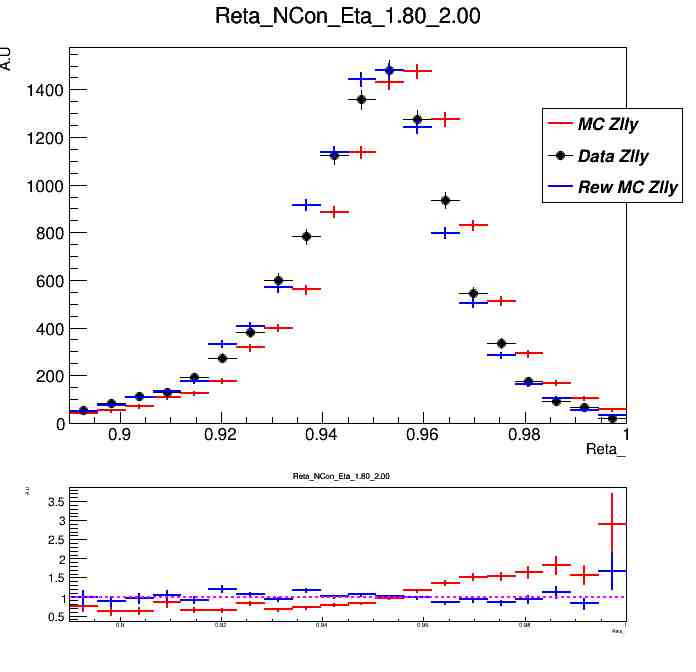
\includegraphics[width=.35\textwidth]{Adx/Adx1/Img/Photon/RetaRew_NCon_Eta_1.80_2.00Zlly.jpg}}
    \caption{The energy profile in $\phi$ and $\eta$ directions (a,b) and the corresponding \Rphi \ and \Reta \ variables, for unconverted photons with 1.80$<|\eta|<$2.00. The black points correspond to the pseudo data, red points to non-reweighted simulation and blue points to the reweighted simulation from $Z\rightarrow ll\gamma$ with derived photon reweighting.}
    \label{Photon:2}
\end{figure}

\begin{figure}[ht]
    \centering
	\subfloat[][]{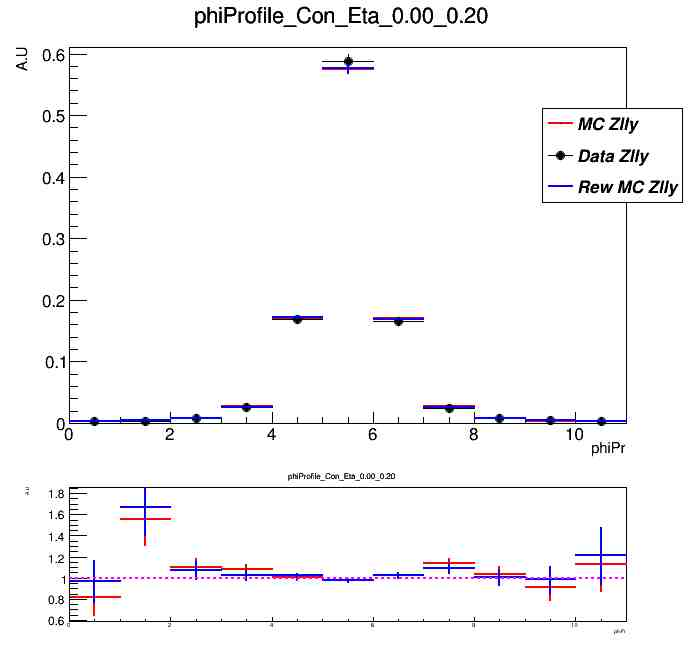
\includegraphics[width=.35\textwidth]{Adx/Adx1/Img/Photon/phiProfileRew_Con_Eta_0.00_0.20Zlly.jpg}}
	\subfloat[][]{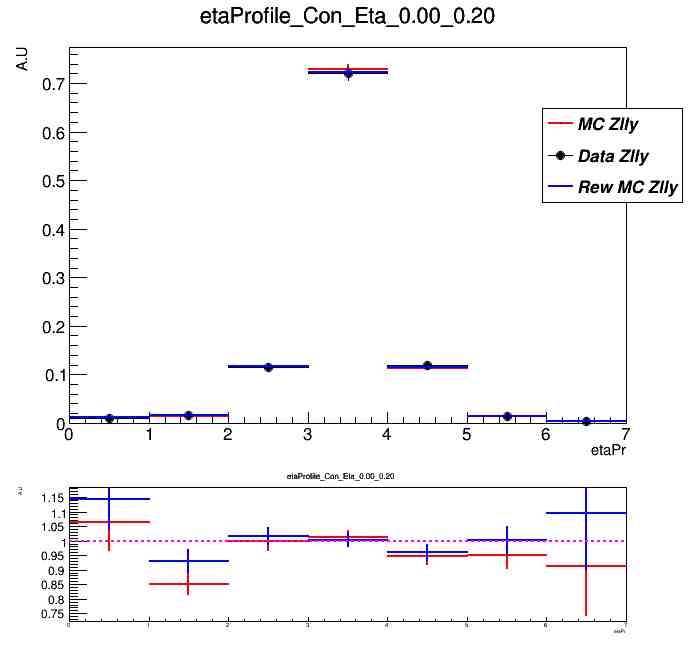
\includegraphics[width=.35\textwidth]{Adx/Adx1/Img/Photon/etaProfileRew_Con_Eta_0.00_0.20Zlly.jpg}} \\
	\subfloat[][]{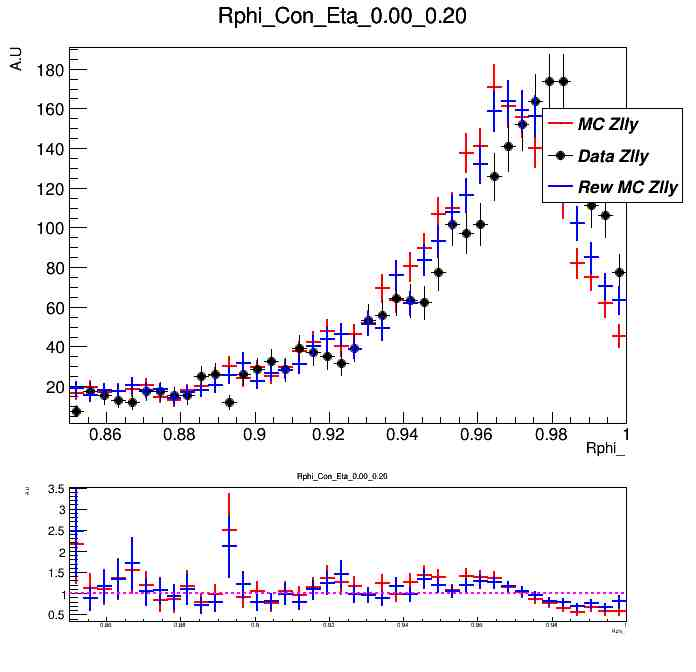
\includegraphics[width=.35\textwidth]{Adx/Adx1/Img/Photon/RphiRew_Con_Eta_0.00_0.20Zlly.jpg}}
	\subfloat[][]{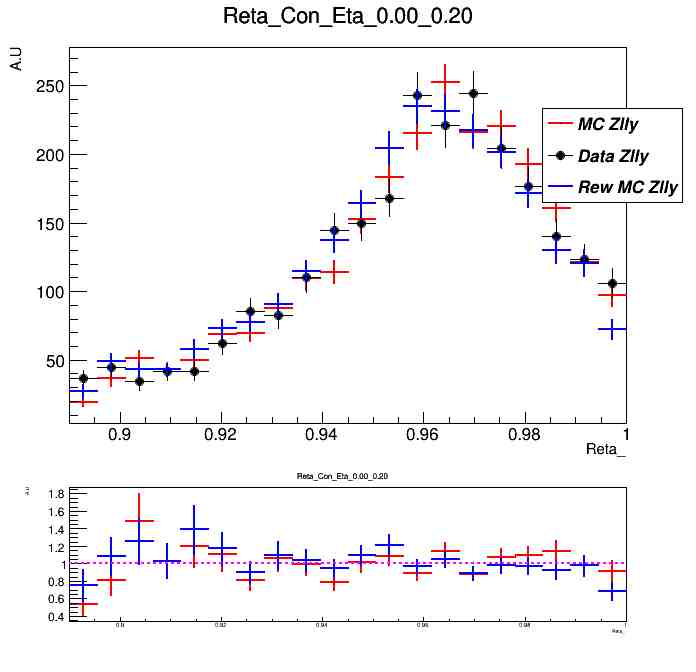
\includegraphics[width=.35\textwidth]{Adx/Adx1/Img/Photon/RetaRew_Con_Eta_0.00_0.20Zlly.jpg}}
    \caption{The energy profile in $\phi$ and $\eta$ directions (a,b) and the corresponding \Rphi \ and \Reta \ variables, for converted photons with 0.00$<|\eta|<$0.20. The black points correspond to the pseudo data, red points to non-reweighted simulation and blue points to the reweighted simulation from $Z\rightarrow ll\gamma$ with derived photon reweighting.}
    \label{Photon:3}
\end{figure}

\begin{figure}[ht]
    \centering
	\subfloat[][]{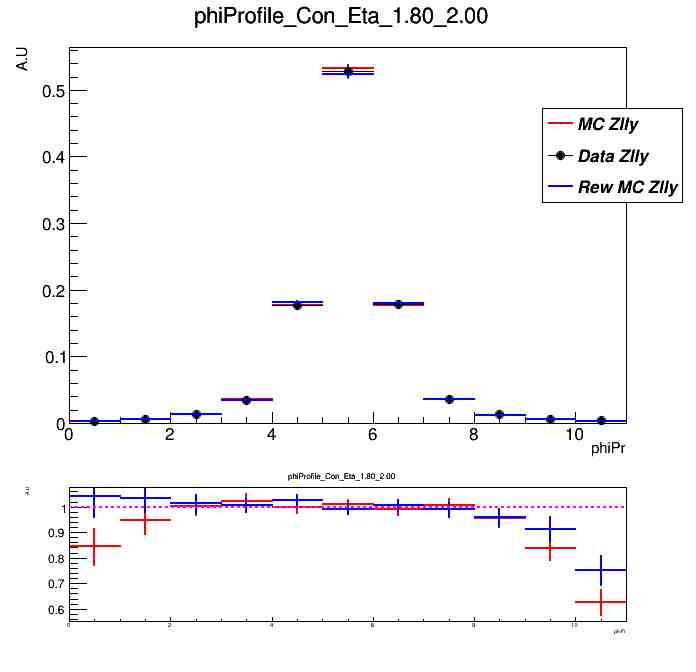
\includegraphics[width=.35\textwidth]{Adx/Adx1/Img/Photon/phiProfileRew_Con_Eta_1.80_2.00Zlly.jpg}}
	\subfloat[][]{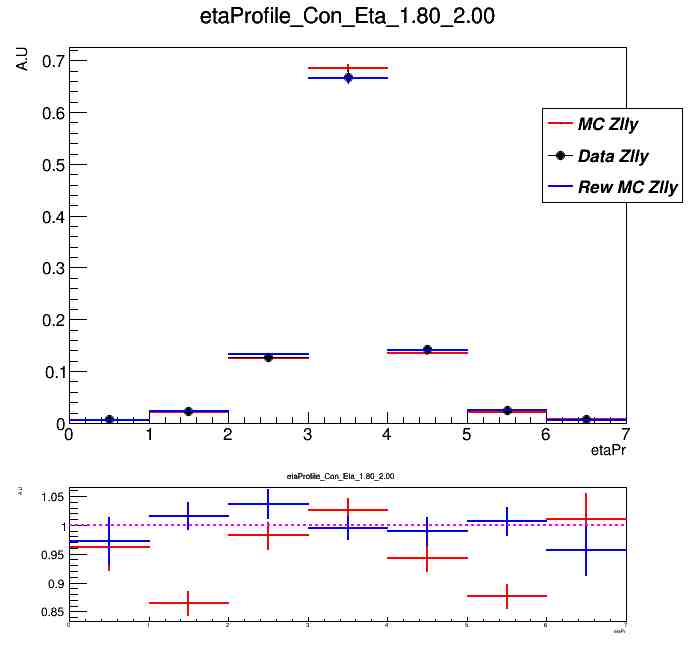
\includegraphics[width=.35\textwidth]{Adx/Adx1/Img/Photon/etaProfileRew_Con_Eta_1.80_2.00Zlly.jpg}} \\
	\subfloat[][]{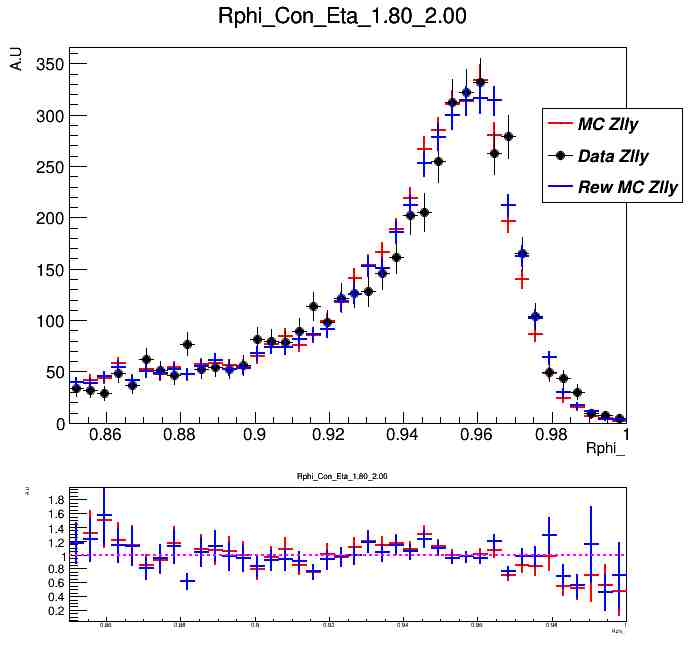
\includegraphics[width=.35\textwidth]{Adx/Adx1/Img/Photon/RphiRew_Con_Eta_1.80_2.00Zlly.jpg}}
	\subfloat[][]{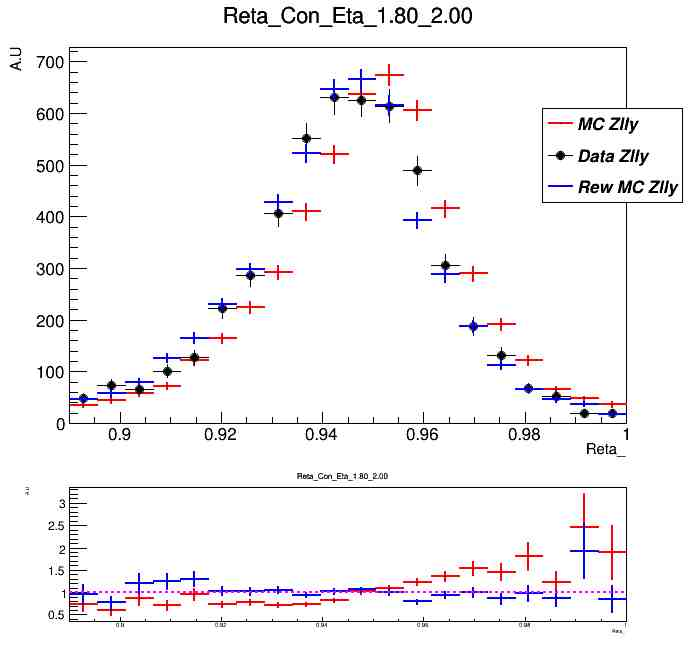
\includegraphics[width=.35\textwidth]{Adx/Adx1/Img/Photon/RetaRew_Con_Eta_1.80_2.00Zlly.jpg}}
    \caption{The energy profile in $\phi$ and $\eta$ directions (a,b) and the corresponding \Rphi \ and \Reta \ variables, for converted photons with 1.80$<|\eta|<$2.00. The black points correspond to the pseudo data, red points to non-reweighted simulation and blue points to the reweighted simulation from $Z\rightarrow ll\gamma$ with derived photon reweighting.}
    \label{Photon:4}
\end{figure}

